% This is a LaTeX thesis template for Adam Mickiewicz University.
% to be used with quarto
% This template was produced by Jakub Nowosad
% Version: 22 July 2023

% Inspired by:
% This is a LaTeX thesis template for Monash University.
% to be used with Rmarkdown
% This template was produced by Rob Hyndman
% Version: 6 September 2016

\documentclass{amuthesis}
% \usepackage[polish]{babel}
\usepackage{polski}
\renewcommand{\figurename}{Rycina} % Redefine default figure caption %
\renewcommand{\tablename}{Tabela} % Redefine default table caption %
%%%%%%%%%%%%%%%%%%%%%%%%%%%%%%%%%%%%%%%%%%%%%%%%%%%%%%%%%%%%%%%
% Add any LaTeX packages and other preamble here if required
%%%%%%%%%%%%%%%%%%%%%%%%%%%%%%%%%%%%%%%%%%%%%%%%%%%%%%%%%%%%%%%
\usepackage{booktabs,tabularx} % Allows kableExtra to work %
\usepackage{indentfirst} % Adds indent in the first paragraph %
\usepackage{bookmark} % Adds indent in the first paragraph %

\author{Filip Ratajszczak}
\title{Wykrywanie farm fotowoltaicznych na podstawie danych
teledetekcyjnych}
\def\titleeng{Detection of photovoltaic farms based on remote sensing
data}
\def\degreetitle{Praca inżynierska}
\def\major{Geoinformacja}
\def\albumid{461791}
\def\thesisyear{2024}

% Add subject and keywords below
\hypersetup{
     %pdfsubject={The Subject},
     %pdfkeywords={Some Keywords},
     pdfauthor={Filip Ratajszczak},
     pdftitle={Wykrywanie farm fotowoltaicznych na podstawie danych
teledetekcyjnych},
     pdfproducer={quarto with LaTeX}
}

\bibliography{thesis.bib, packages.bib}

\begin{document}

\pagenumbering{arabic}

\titlepage

\bookmarksetup{startatroot}

\hypertarget{streszczenie}{%
\chapter*{Streszczenie}\label{streszczenie}}
\addcontentsline{toc}{chapter}{Streszczenie}

\markboth{Streszczenie}{Streszczenie}

\textbf{Abstrakt}

Streszczenie powinno przedstawiać skrótowo główny problem pracy i jego
rozwiązanie. Możliwa struktura streszczenia to: (1) 1-3 zdania wstępu do
problemu (czym się zajmujemy, dlaczego jest to ważne, jakie są
problemy/luki do wypełnienia), (2) 1 zdanie opisujące cel pracy, (3) 1-3
zdania przedstawiające użyte materiały (dane) i metody (techniki,
narzędzia), (4) 1-3 zdania obrazujące główne wyniki pracy, (5) 1-2
zdania podsumowujące; możliwe jest też określenie dalszych
kroków/planów.

Słowa kluczowe: (4-6 słów/zwrotów opisujących treść pracy, które nie
wystąpiły w tytule)

\textbf{Abstract}

The abstract must be consistent with the above text.

Keywords: (as stated before)

\newpage

\setstretch{1.2}\sf\tighttoc\doublespacing

\bookmarksetup{startatroot}

\hypertarget{sec-wprowadzenie}{%
\chapter{Wprowadzenie}\label{sec-wprowadzenie}}

Wprowadzenie powinno mieć charakter opisu od ogółu do szczegółu (np.
trzy-pięć paragrafów). Pierwszy paragraf powinien być najbardziej
ogólny, a kolejne powinny przybliżać czytelnika do problemu.
Przedostatni paragraf powinien określić jaki jest problem (są problemy),
który praca ma rozwiązać i dlaczego jest to (są one) ważne.

Wprowadzenie powinno być zakończone stwierdzeniem celu pracy. Dodatkowo
tutaj może znaleźć się również krótki opis co zostało zrealizowane w
pracy.

\bookmarksetup{startatroot}

\hypertarget{sec-lit}{%
\chapter{Przegląd literatury}\label{sec-lit}}

\bookmarksetup{startatroot}

\hypertarget{sec-materialy}{%
\chapter{Materiały}\label{sec-materialy}}

\begin{figure}[t]

{\centering 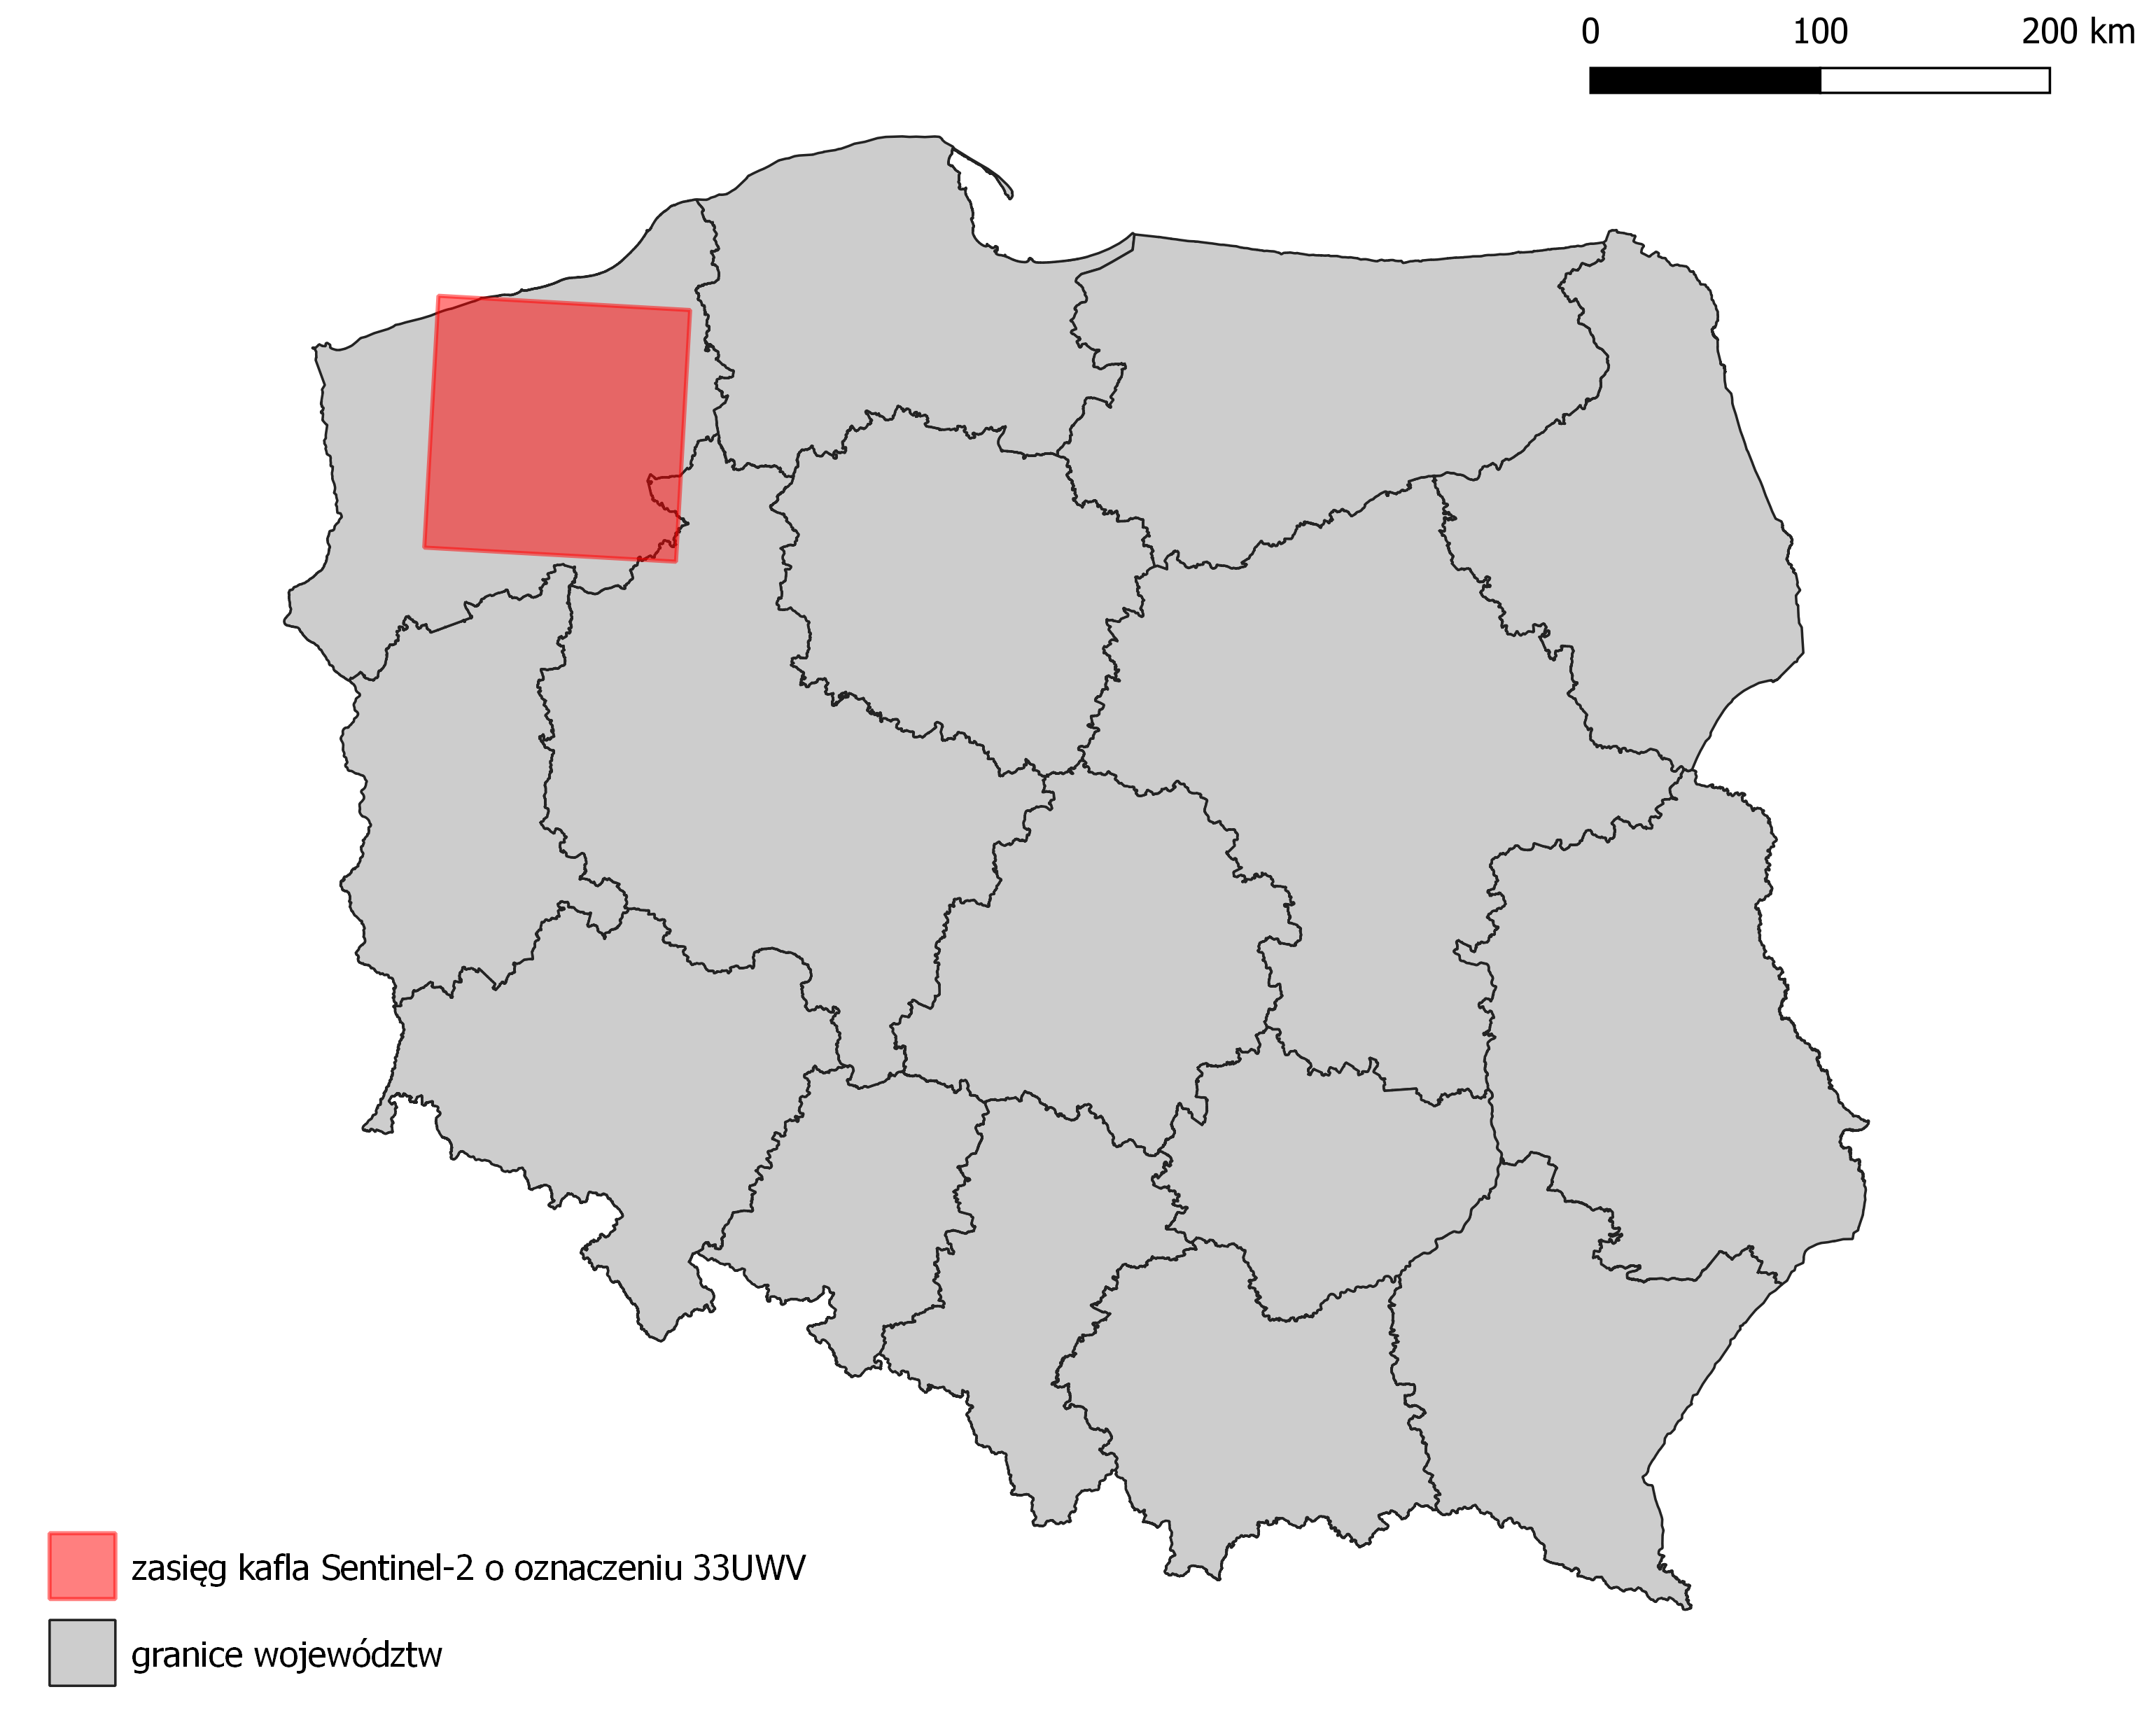
\includegraphics[width=1\textwidth,height=\textheight]{figures/sen2_extent.png}

}

\caption{\label{fig-rycina-area}Obszar badań}

\end{figure}

\hypertarget{sec-satellite-imagery}{%
\section{Zdjęcia satelitarne}\label{sec-satellite-imagery}}

\hypertarget{sec-sentinel1}{%
\subsection{Sentinel-1}\label{sec-sentinel1}}

Sentinel-1 to wspólna inicjatywa Komisji Europejskiej i Europejskiej
Agencji Kosmicznej w ramach programu Copernicus, mająca na celu
dostarczanie danych radarowych obejmujących globalną powierzchnię Ziemi,
w tym lądów, europejskich stref przybrzeżnych, tras żeglugowych, stref
lodu morskiego, mórz i oceanów
\autocite{hejmanowska_2020_dane,sentinel1_mission_objectives}. Misja
odpowiada na potrzeby monitorowania obszarów morskich i lądowych, w tym
przemieszczania kry lodowej, transportu morskiego, deformacji i
przemieszczeń terenu, a także obserwacji zmian klimatu i klęsk
żywiołowych
\autocite{hejmanowska_2020_dane,sentinel1_mission_objectives}.

Sentinel-1 posiada pojedynczy radar z syntetyzowaną aperturą (ang.
\emph{Synthetic Aperture Radar}, SAR), który działa na jednej
częstotliwości środkowej 5,405 GHz, co odpowiada długości fali 5,6 cm
\autocite{sentinel1_lulc,sentinel1_instrument_payload}. Częstotliwość
radaru Sentinel-1, mieszcząca się w pasmie C (od 4 do 8 GHz),
determinuje jego zdolność do penetracji jedynie górnych warstw koron
drzew, roślinności oraz gleby \autocite{sentinel_1_user_guide}. Radar
jest najczęściej wykorzystywany w trybie podwójnej polaryzacji, emitując
fale pionowe i mierząc zarówno fale pionowe (ang. \emph{vertical}), jak
i poziome (ang. \emph{horizontal}) po ich powrocie do czujnika, dzięki
czemu otrzymujemy dane o intensywności rozproszenia wstecznego VV i VH
\autocite{sentinel1_lulc}. Radar z syntetyzowaną aperturą (SAR)
umożliwia prowadzenie obserwacji zarówno w nocy, jak i w dzień,
niezależnie od warunków pogodowych, przez co czas rewizyty konstelacji
dwóch satelitów dla obszaru Polski wynosi około 2 dni
\autocite{attema_2008_s1,sentinel1_revisit}. W grudniu 2021 roku w
satelicie Sentinel-1B wystąpiła anomalia związana z zasilaniem
elektroniki radaru, uniemożliwiająca dalsze dostarczanie danych
radarowych \autocite{sentinel_1b}. W wyniku awarii satelita Sentinel-1B
został wyłączony z użytku, a wystrzelenie platformy Sentinel-1C
zaplanowano na marzec 2024 roku
\autocite{sentinel_1b,sentinel1_eoportal}.

Dane radarowe Sentinel-1 sa dostępne na trzech poziomach przetworzenia.
Produkty poziomu 1 (Single Look Complex (SLC) i Ground Range Detected
(GRD)), są przeznaczone dla użytkowników końcowych i nadają się, w
zależności od produktu do monitorowania Ziemi, klasyfikacji pokrycia
terenu czy aplikacji interferometrycznych
\autocite{hejmanowska_2020_dane}. Interferometria radarowa (ang.
\emph{Interferometric Synthetic Aperture Radar}, InSAR) to technika
umożliwiająca generowanie cyfrowych modeli wysokościowych (ang.
\emph{digital elevation model}, DEM) oraz pomiary deformacji terenu na
podstawie informacji o fazie sygnału
\autocite{hanssen_2001_insar,hejmanowska_2020_dane}. SLC to obrazy SAR w
geometrii ukośnej, posiadające informację o wartości amplitudy i fazie
sygnału \autocite{hejmanowska_2020_dane}. Produkty GRD są rezultatem
przepróbkowania obrazów SLC do jednolitej rozdzielczości przestrzennej
(10 × 10 m) i rzutowania na powierzchnię elipsoidy odniesienia
\autocite{hejmanowska_2020_dane}. GRD nie zawiera cech ortofotomapy i
wymaga dodatkowego przepróbkowania z użyciem numerycznego modelu terenu
przed zastosowaniem w systemach GIS \autocite{hejmanowska_2020_dane}.
Przy konwersji SLC do GRD tracimy informację fazową sygnału, co sprawia,
że produkty GRD nie są odpowiednie do interferometrii radarowej
\autocite{sentinel1_products}.

Dane Sentinel-1 rejestrowane są w czterech trybach: Interferometric Wide
Swath (IW) - podstawowy tryb obrazowania dla obszarów lądowych, Stripmap
(SM) - używany do obrazowania małych wysp i na potrzeby zarządzania
kryzysowego, Extra-Wide Swath (EW) - tryb do monitorowania stref
polarnych i niektórych obszarów morskich oraz Wave (WV) - tryb
obrazowania oceanów
\autocite{hejmanowska_2020_dane,sentinel1_instrument_payload,sentinel1_stripmap}.
Charakterystykę konkretnych trybów akwizycji radaru Sentinel-1
przedstawia tabela \ref{tbl-tabela-sentinel1}
\autocite{sentinel1_resolution_swath}.

\hypertarget{tbl-tabela-sentinel1}{}
\begin{table}
\caption{\label{tbl-tabela-sentinel1}Tryby radaru Sentinel-1
(\href{https://sentinels.copernicus.eu/web/sentinel/missions/sentinel-1/instrument-payload/resolution-swath}{ESA,
2023}) }\tabularnewline

\centering
\begin{tabular}{>{\centering\arraybackslash}p{3cm}>{\centering\arraybackslash}p{1.8cm}>{\centering\arraybackslash}p{2.4cm}>{\centering\arraybackslash}p{2.8cm}>{\centering\arraybackslash}p{2cm}}
\toprule
Tryb & Kąt padania wiązki [°] & Rozdzielczość przestrzenna [m] & Szerokość rejestrowanego pasa [km] & Polaryzacje (H=pozioma, V=pionowa)\\
\midrule
Stripmap & 20 - 45 & 5 x 5 & 80 & HH+HV, VH+VV, HH, VV\\
\addlinespace
\textbf{Interferometric Wide Swath} & \textbf{29 - 46} & \textbf{5 x 20} & \textbf{250} & \textbf{HH+HV, VH+VV, HH, VV}\\
\addlinespace
Extra Wide Swath & 19 - 47 & 20 x 40 & 400 & HH+HV, VH+VV, HH, VV\\
\addlinespace
Wave & 22 - 35   35 - 38 & 5 x 5 & 20 x 20 & HH, VV\\
\bottomrule
\end{tabular}
\end{table}

W pracy wykorzystano dwie polaryzacje (VV i VH) pochodzące z produktów
Ground Range Detected (GRD), zarejestrowanych w trybie Interferometric
Wide Swath (IW) przez platformę Sentinel-1A w dniu 8 maja 2023 roku.
Użyty zestaw danych został utworzony poprzez połączenie dwóch sąsiednich
produktów Sentinel-1 GRD, a następnie ograniczenie obszaru analizy do
kafla Sentinel-2 o oznaczeniu 33UWV.

\hypertarget{sec-sentinel2}{%
\subsection{Senitnel-2}\label{sec-sentinel2}}

Misja Sentinel-2 stanowi inicjatywę Komisji Europejskiej, która jest
operacyjnie prowadzona przez Europejską Agencję Kosmiczną (ang.
\emph{European Space Agency}, ESA) w ramach programu Copernicus. Celem
tej misji jest dostarczanie obrazów satelitarnych, obejmujących
trzynaście zakresów spektralnych o różnych rozdzielczościach
przestrzennych: 10, 20 lub 60 metrów, zależnie od rejestrowanego kanału.
Czas rewizyty konstelacji dwóch satelitów wzrasta z 5 dni nad równikiem
do 2-3 dni na średnich szerokościach geograficznych, obejmujących obszar
Polski \autocite{hejmanowska_2020_dane,sentinel_2_guide}.

Dane pozyskiwane przez satelity Sentinel-2 są dostępne na różnych
poziomach przetworzenia, lecz najczęściej używane przy tworzeniu map
pokrycia terenu i użytkowania ziemi (ang. \emph{Land Use/Land Cover},
LULC) są produkty 1C (współczynnik odbicia na poziomie górnej części
atmosfery; ang. \emph{Top-of-Atmospheric reflectance}, TOA) oraz 2A
(współczynnik odbicia na powierzchni Ziemi; ang.
\emph{Bottom-of-Atmospheric reflectance}, BOA)
\autocite{phiri_2020_sentinel2}.

Produkty poziomu 1C to dane poddane korekcjom radiometrycznym i
geometrycznym, prezentowane jako sceny o powierzchni 100
km\textsuperscript{2} (100 x 100 km) w projekcji UTM/WGS84
\autocite{esa_2015_sentinel2handbook}. Skuteczne wykorzystanie tych
danych w zastosowaniach związanych z terenami lądowymi wymaga
precyzyjnej korekcji zdjęć satelitarnych pod kątem efektów
atmosferycznych \autocite{main-knorn_2017_Sen2Cor}. Produkty poziomu 2A
powstają poprzez zastosowanie dodatkowej korekcji atmosferycznej dla
danych poziomu 1C za pomocą procesora korekcji atmosferycznej Sen2Cor
\autocite{main-knorn_2017_Sen2Cor}.

\hypertarget{tbl-tabela-sentinel2}{}
\begin{table}
\caption{\label{tbl-tabela-sentinel2}Kanały spektralne satelitów Sentinel-2
(\href{https://sentinels.copernicus.eu/web/sentinel/user-guides/sentinel-2-msi/resolutions/spectral}{ESA,
2023}) }\tabularnewline

\centering
\begin{tabular}{>{\centering\arraybackslash}p{1.5cm}>{\centering\arraybackslash}p{4cm}>{\centering\arraybackslash}p{2cm}>{\centering\arraybackslash}p{2cm}>{\centering\arraybackslash}p{2.4cm}}
\toprule
Kanał & Nazwa kanału & Centralna długość fali [nm] & Zakres spektralny [nm] & Rozdzielczość przestrzenna [m]\\
\midrule
B01 & Coastal Aerosol & 443 & 433–453 & 60\\
\textbf{B02} & \textbf{Blue} & \textbf{493} & \textbf{458–523} & \textbf{10}\\
\textbf{B03} & \textbf{Green} & \textbf{560} & \textbf{543–578} & \textbf{10}\\
\textbf{B04} & \textbf{Red} & \textbf{665} & \textbf{650–680} & \textbf{10}\\
\textbf{B05} & \textbf{Vegetation RedEdge} & \textbf{704} & \textbf{698–713} & \textbf{20}\\
\textbf{B06} & \textbf{Vegetation RedEdge} & \textbf{740} & \textbf{733–748} & \textbf{20}\\
\textbf{B07} & \textbf{Vegetation RedEdge} & \textbf{783} & \textbf{773–793} & \textbf{20}\\
\textbf{B08} & \textbf{NIR} & \textbf{833} & \textbf{785–900} & \textbf{10}\\
\textbf{B8A} & \textbf{NIR} & \textbf{865} & \textbf{855–875} & \textbf{20}\\
B09 & Water Vapour & 945 & 935–955 & 60\\
B10 & Cirrus & 1374 & 1360–1390 & 60\\
\textbf{B11} & \textbf{SWIR} & \textbf{1610} & \textbf{1565–1655} & \textbf{20}\\
\textbf{B12} & \textbf{SWIR} & \textbf{2190} & \textbf{2100–2280} & \textbf{20}\\
\bottomrule
\end{tabular}
\end{table}

Dane wykorzystane w analizie pochodzą z dnia 8 maja 2023 roku i zostały
dostarczone przez satelitę Sentinel-2B. Obszar analizy obejmuje kafel
(ang. \emph{tile}) o oznaczeniu 33UWV, dla którego współczynnik
zachmurzenia w tym dniu wynosił 0,7\%. Użyte zostały dane na poziomie
przetworzenia L2A. Z dostępnych kanałów spektralnych (tabela
\ref{tbl-tabela-sentinel2} \autocite{sentinel_2_user_guide})
wykorzystano 10 zakresów, ponieważ pasma rejestrowane w rozdzielczości
60 metrów są przeznaczone głównie do korekcji atmosferycznych i detekcji
chmur. Kanał 1 (443 nm) służy do korekcji wpływu aerozoli, kanał 9 (940
nm) do korekcji wpływu pary wodnej, a kanał 10 (1375 nm) do wykrywania
chmur typu cirrus \autocite{drusch_2012_sen2GMES}.

\hypertarget{sec-mosaics}{%
\section{Ortofotomapa i mozaiki zdjęć satelitarnych}\label{sec-mosaics}}

Do lokalizacji oraz wektoryzacji istniejących farm fotowoltaicznych
wykorzystano ortofotomapę udostępnianą przez Główny Urząd Geodezji i
Kartografii (GUGiK) oraz mozaiki zdjęć satelitarnych dostarczane przez
podmioty komercyjne. W teledetekcji jednym z zastosowań mozaik obrazów
satelitarnych jest tworzenie zestawów danych referencyjnych poprzez
interpretację wizualną, np. w celu walidacji wyników klasyfikacji
produktów pokrycia terenu \autocite{lesiv_2018_sat_imagery_mosaics}. Do
stworzenie zbioru danych testowych i treningowych wykorzystano
ortomozaiki Google Satellite, Bing Aerial oraz Planet Basemaps,
udostępniane w formie usług sieciowych (WMS, WMTS, XYZ Tiles). Mozaiki
te są tworzone na podstawie komercyjnych zdjęć satelitarnych
wykonywanych przez podmioty takie jak Maxar Technologies, Airbus czy
Planet Labs.

Większość ortofotomap dostarczanych przez GUGiK jest zrealizowana w
standardzie 25 x 25 cm, jednakże na obszarach miejskich charakteryzują
się one rozdzielczością przestrzenną wynoszącą 10 cm lub nawet wyższą
\autocite{ortofotomapa}. Rozdzielczość przestrzenna wykorzystanych
mozaik obrazów satelitarnych (oprócz Planet Basemaps) jest wyższa niż 1
m, na przykład mozaika Bing Aerial dostarczana przez firmę Microsoft
cechuje się wielkością komórki od 30 do 60 cm \autocite{bing_aerial}.
Często jednak nie jest możliwie ustalenie dat wykonania zdjęć
satelitarnych, które posłużyły do stworzenia konkretnej mozaiki
zobrazowań satelitarnych \autocite{lesiv_2018_sat_imagery_mosaics}.
Mozaika tworzona przez Planet na podstawie zdjęć satelitarnych
wykonywanych przez konstelację satelitów PlanetScope charakteryzuje się
rozdzielczością przestrzenną 4,77 m na równiku, jednak w porównaniu do
pozostałych wymienionych produktów jest tworzona z miesięczną oraz
kwartalną częstotliwością \autocite{planet_2019_basemaps}. Pozwala to,
pomimo niższej rozdzielczości przestrzennej na stworzenie zbioru danych
testowych i treningowych na konkretny okres czasu. Mozaiki Planet
Basemaps są tworzone na podstawie najlepszych obrazów z katalogu Planet
w określonym przedziale czasowym, co umożliwia generowanie
wysokorozdzielczych mozaik, które są dokładne radiometrycznie i
przestrzennie, a także charakteryzują się zminimalizowanym wpływem
czynników atmosferycznych \autocite{planet_2019_basemaps}.

\begin{figure}[t]

{\centering 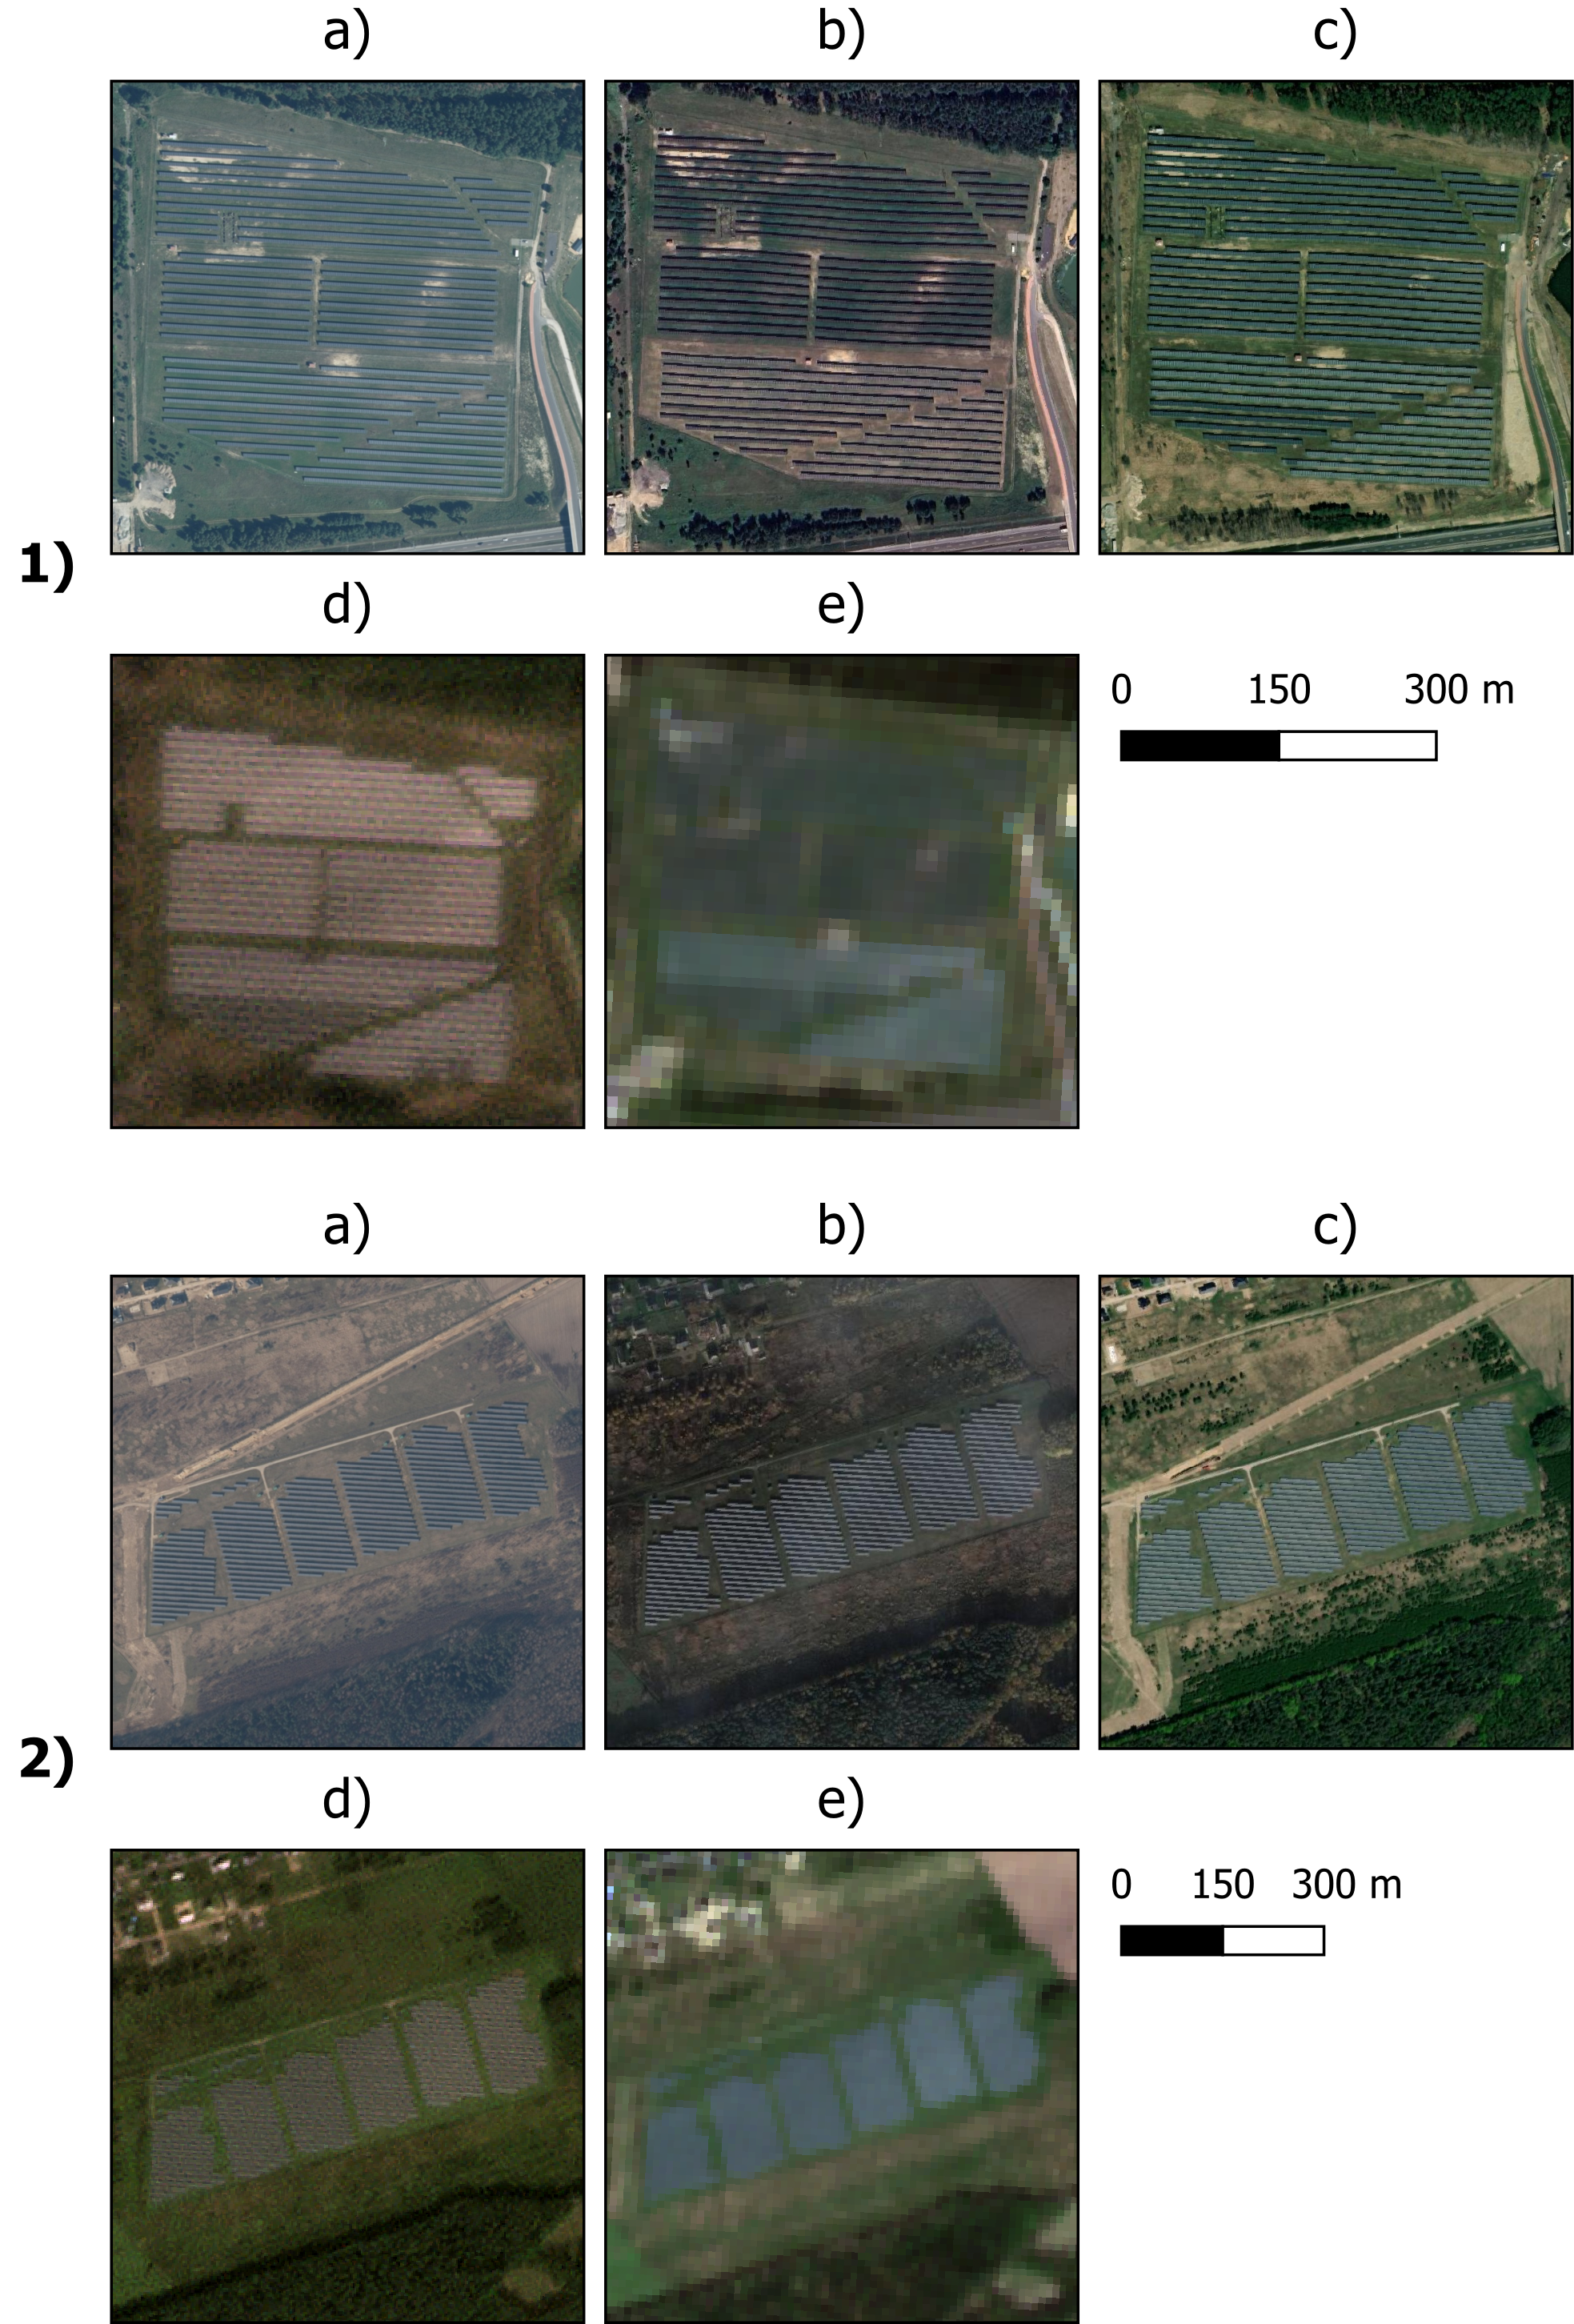
\includegraphics[width=1\textwidth,height=\textheight]{figures/pv.png}

}

\caption{\label{fig-rycina-pv}Porównanie wyglądu farm fotowoltaicznych w
Kulicach k. Nowogardu (1) i Wałczu (2) na ortofotomapie udostępnianej
przez GUGiK (a), Google Satellite (b), Bing Aerial (c), Planet Basemaps
(d) oraz w kompozycji RGB Sentinel-2 (e)}

\end{figure}

\bookmarksetup{startatroot}

\hypertarget{sec-metody}{%
\chapter{Metody}\label{sec-metody}}

\hypertarget{sec-processing}{%
\section{Przygotowanie danych}\label{sec-processing}}

\hypertarget{sec-processing-s1}{%
\subsection{Sentinel-1}\label{sec-processing-s1}}

Korzystanie z danych radarowych wymaga wcześniejszego przygotowania
danych poprzez proces kalibracji, aby zapewnić poprawne wyniki analizy.
Procesy te mogą różnić się w zależności od konkretnego zastosowania,
mając na celu dostosowanie danych do specyficznych potrzeb. W pracy
wykorzystano schemat przetwarzania danych Sentinel-1 GRD, który
zaproponował \textcite{filipponi_2019_s1_workflow}, obejmujący:

\begin{enumerate}
\def\labelenumi{\arabic{enumi}.}
\item
  aktualizację informacji o położeniu satelity w momencie zobrazowania
  poprzez pobranie dokładnych wektorów stanu orbity dla produktu
  zapewniając precyzyjne informacje o pozycji i prędkości satelity
  podczas akwizycji;
\item
  korekcję szumów termicznych;
\item
  korekcję szumów na granicach obrazów;
\item
  obliczenie współczynnika rozproszenia wstecznego (ang.
  \emph{backscatter coefficient}) sigma0 za pomocą kalibracji
  radiometrycznej;
\item
  korekcję topograficzną (ortorektyfikacja za pomocą Copernicus 30 m
  Global DEM);
\item
  konwersję współczynnika rozproszenia wstecznego na dB za pomocą
  transformacji logarytmicznej
\end{enumerate}

\begin{figure}[t]

{\centering 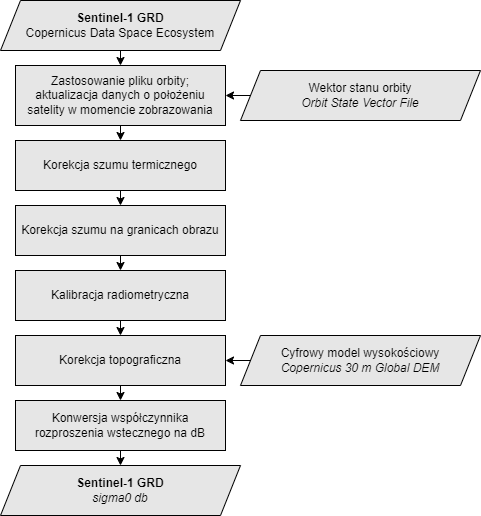
\includegraphics[width=5.01042in,height=5.38542in]{figures/sentinel1_workflow.drawio.png}

}

\caption{\label{fig-rycina-s1-workflow}Przebieg wstępnego przetwarzania
danych Sentinel-1 Ground Range Detected (GRD)}

\end{figure}

Wstępne przetwarzanie danych dla obu wykorzystywanych polaryzacji (VV i
VH) zostało wykonane przy użyciu zestawu narzędzi ESA Sentinel-1 Toolbox
(S1TBX) \autocite{s1tbx} w oprogramowaniu SNAP \autocite{snap} przy
pomocy narzędzia do przetwarzania grafów (ang. \emph{Graph Processing
Tool}, GPT) . Kolejne etapy przygotowania danych zostały zrealizowane
przy wykorzystaniu języka R (\textcite{R-base}) oraz pakietu
\emph{terra} \autocite{R-terra}. Obszar analizy, będący kaflem
Sentinel-2 o oznaczeniu 33UWV, znajduje się na granicy dwóch sąsiednich
produktów Sentinel-1 GRD. Na potrzeby dalszego przetwarzania,
sąsiadujące produkty zostały połączone i odpowiednio ograniczone do
obszaru zainteresowania. Na granicy sąsiednich produktów Sentinel-1 GRD
występowała przestrzeń bez danych o szerokości jednej komórki, co
wymagało wypełnienia tego obszaru danymi przy użyciu funkcji
\texttt{focal} z pakietu \emph{terra} \autocite{R-terra}.

\begin{figure}[t]

{\centering 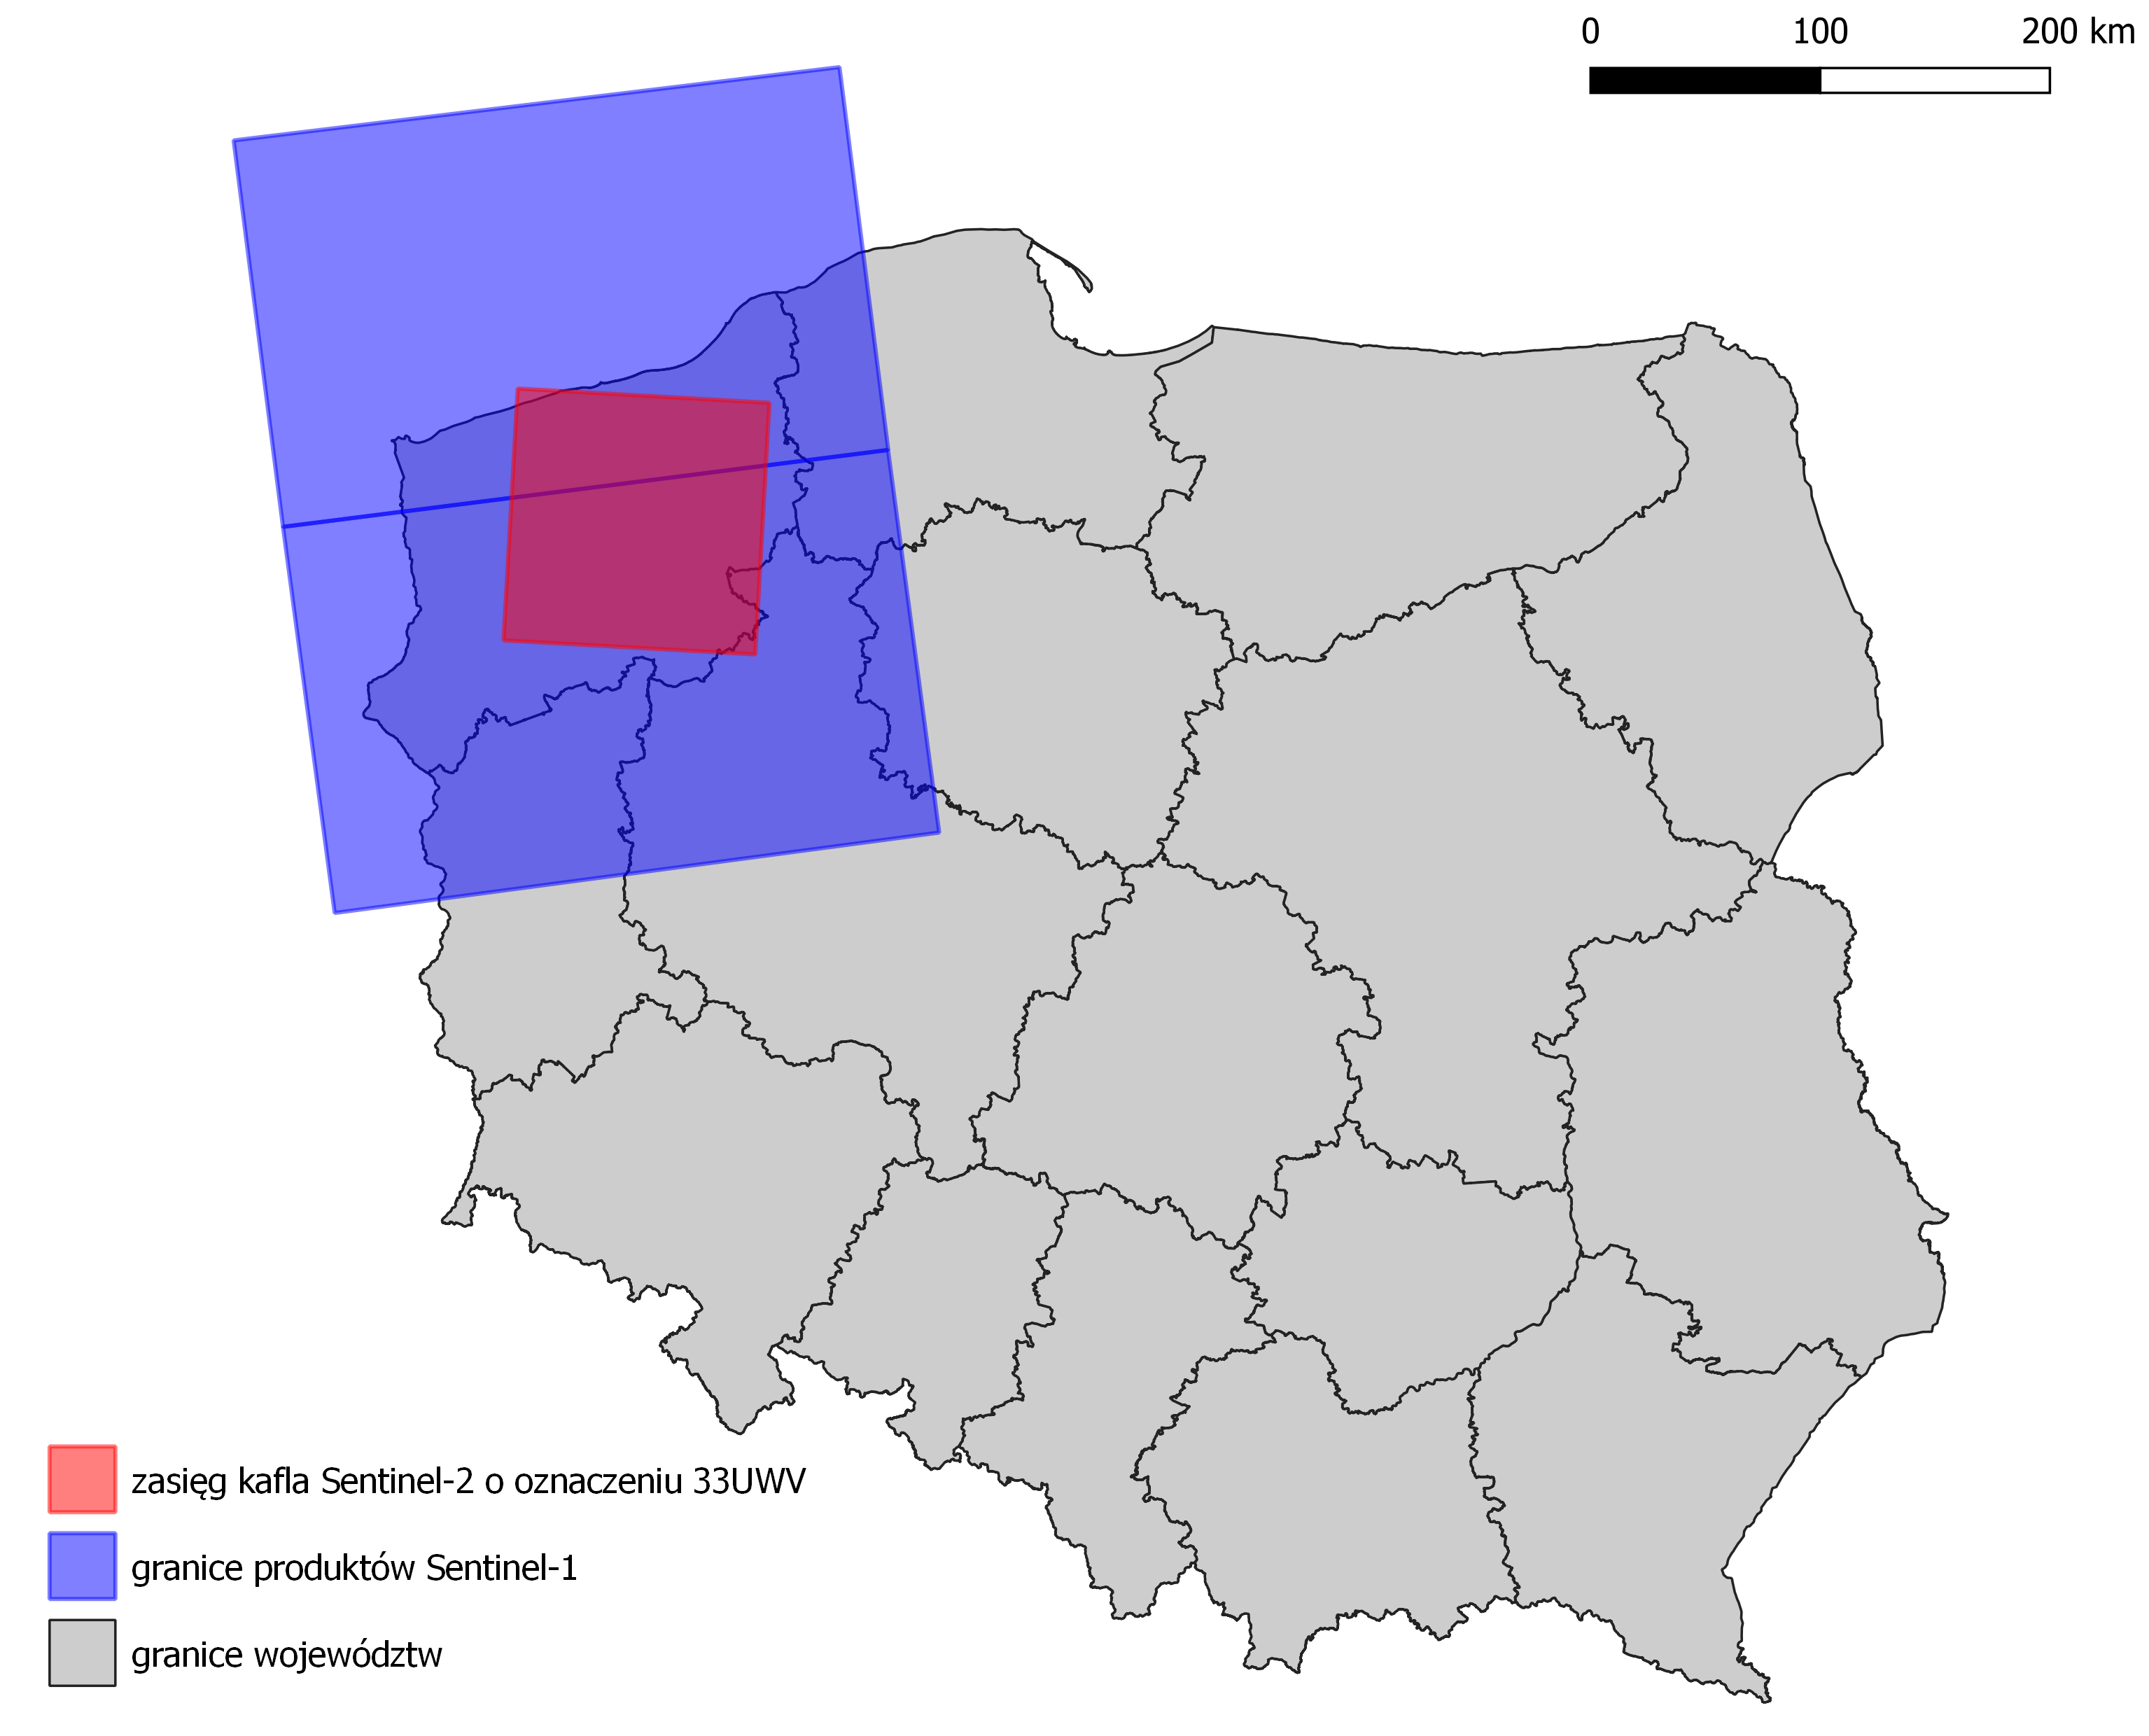
\includegraphics[width=1\textwidth,height=\textheight]{figures/sen1_extents.png}

}

\caption{\label{fig-rycina-s1-extents}Obszar badań i zasięg
wykorzystanych produktów Sentinel-1}

\end{figure}

\hypertarget{sec-processing-s2}{%
\subsection{Sentinel-2}\label{sec-processing-s2}}

Przetwarzanie danych Sentinel-2 polegało na sprowadzeniu kanałów o
rozdzielczości 20 m do rozdzielczości i siatki kanałów w rozdzielczości
10 m. Przepróbkowanie (ang. \emph{resampling}) zostało przeprowadzone
przy pomocy funkcji \texttt{resample} z pakietu \emph{terra}
\autocite{R-terra}, stosując interpolację dwuliniową (ang.
\emph{bilinear interpolation}).

\hypertarget{sec-spectral-indices}{%
\subsection{Wskaźniki spektralne}\label{sec-spectral-indices}}

Oprócz surowych współczynników odbicia, w niektórych wariantach
predykcji zastosowano również wskaźniki spektralne (ang. \emph{spectral
indices}), które były wykorzystywane w poprzednich badaniach dotyczących
detekcji farm fotowoltaicznych na podstawie danych teledetekcyjnych
przez \textcite{zhang_2021_texture}, \textcite{plakman_2022_pv},
\textcite{wang_2022_pv} i innych, takie jak:

\begin{itemize}
\item
  znormalizowany różnicowy wskaźnik wegetacji (ang. \emph{Normalized
  Difference Vegetation Index}, NDVI) \autocite{ndvi}, monitorujący
  zawartość biomasy i kondycję roślinności na danym obszarze:

  \[
  NDVI = \frac{NIR - Red}{NIR + Red}
  \]

  , gdzie \(NIR\) -- reflektancja w kanale bliskiej podczerwieni,
  \(Red\) -- reflektancja w kanale czerwonym
\item
  znormalizowany różnicowy wskaźnik obszarów zabudowanych (ang.
  \emph{Normalized Difference Built-up Index}, NDBI) \autocite{ndbi},
  przeznaczony do kartowania obszarów zabudowanych:

  \[
  NDBI = \frac{SWIR1 - NIR}{SWIR1 + NIR}
  \]

  , gdzie \(SWIR1\) -- reflektancja w kanale średniej podczerwieni,
  \(NIR\) -- reflektancja w kanale bliskiej podczerwieni
\item
  znormalizowany zmodyfikowany różnicowy wskaźnik wody (ang.
  \emph{Modified Normalized Difference Water Index}, mNDWI)
  \autocite{mndwi}, który skutecznie identyfikuje obszary wodne na
  zdjęciach satelitarnych, posiadając możliwości tłumienia zakłóceń
  spowodowanych przez zabudowę, roślinność i gleby:

  \[
  mNDWI = \frac{Green - SWIR1}{Green + SWIR1}
  \]

  , gdzie \(Green\) -- reflektancja w kanale zielonym, \(SWIR1\) --
  reflektancja w kanale średniej podczerwieni
\end{itemize}

\hypertarget{sec-textures}{%
\subsection{Tekstury obrazu}\label{sec-textures}}

Tekstura stanowi istotną cechę wykorzystywaną do identyfikacji obiektów
i obszarów zainteresowania na obrazie \autocite{haralick_1973_texture} i
odgrywa ona dużą rolę w interpretacji wizualnej zdjęć lotniczych i
satelitarnych \autocite{lewinski_2012_texture}. Gdy różnice widmowe
pomiędzy klasami są niewielkie, tekstura umożliwia rozróżnienie
odmiennych typów obiektów na podstawie ich organizacji w terenie, często
kontrastując przestrzenie naturalne z antropogenicznymi
\autocite{grass_r_texture}. W zależności od zastosowalnej funkcji
wybrane cechy obrazu zostają uwidocznione w porównaniu z jego obrazem
wejściowym \autocite{lewinski_2012_texture}. Informacja o teksturze może
stanowić dodatkową, przydatną zmienną wejściową w procesach klasyfikacji
lub segmentacji obrazu
\autocite{gong_1992_spatial_features,mumby_2002_ikonos}. Tekstura
obejmuje różnice poziomów szarości (kontrast), obecność lub brak
kierunkowości, regularne wzory i zdefiniowany obszar, na którym
występują zmiany, określony przez rozmiar okna
\autocite{hall_beyer_2017_glcm,grass_r_texture}. Można ją opisać za
pomocą tonu (intensywność poziomu szarości) i struktury (relacje
przestrzenne) \autocite{grass_r_texture}. Model oparty na macierzy
współwystępowania poziomów szarości (ang. \emph{Gray Level Co-Occurrence
Matrix}, GLCM), zaproponowany przez \textcite{haralick_1973_texture},
jest często używany do obliczania tekstur obrazu. Ta metoda polega na
tworzeniu macierzy opisującej częstotliwość występowania par wartości w
określonym fragmencie obrazu, uwzględniając określone sąsiedztwo,
kierunki i odstępy między komórkami \autocite{kupidura_2019_texture}.

Przydatność i wykorzystanie tekstury w dużym stopniu zależy od
rozdzielczości zdjęć satelitarnych i wielkości zjawiska, które
ukształtowało teksturę \autocite{grass_r_texture}. Badanie, które
przeprowadził \textcite{zhang_2021_texture} dotyczące wykorzystania
filtracji teksturalnych w identyfikacji elektrowni fotowoltaicznych z
użyciem Random Forest i danych z Landsata-8 wykazało pozytywny wpływ
tekstur na skuteczność modelu. Według wyników badania najlepiej
dopasowany model wykorzystywał tekstury GLCM o sąsiedztwie 30 pikseli
(co odpowiada wymiarom ruchomego okna o wymiarach 1800 m na 1800 m),
natomiast tekstura o rozmiarze jednego sąsiada ma niewielki wpływ na
poprawę dokładności modelu \autocite{zhang_2021_texture}.

Obliczanie tekstur obrazu może być czasochłonnym procesem, dlatego w
pracy wykorzystano jedynie teksturę średniej sumy (ang. \emph{Sum
Average}, SA lub SAVG), wskazaną przez \textcite{wang_2022_pv} jako
teksturę niosącą najwięcej informacji w kontekście detekcji farm
fotowoltaicznych na podstawie danych Sentinel-1, Sentinel-2 i algorytmu
Random Forest. W celu skrócenia czasu obliczeń, w pracy zdecydowano się
na zastosowanie ruchomego okna o sąsiedztwie 9 komórek.

\hypertarget{sec-processing-data-merging}{%
\subsection{Łączenie danych}\label{sec-processing-data-merging}}

W celu uzyskania spójnych wielokanałowych rastrów, wszystkie zbiory
danych zostały sprowadzone do wspólnej rozdzielczości i siatki.
Rozdzielczość przestrzenna danych Sentinel-1 GRD, analogicznie do danych
Sentinel-2 przegotowanych w sposób przedstawiony w sekcji
\ref{sec-processing-s2} wynosi 10 m. Mimo że rozdzielczość przestrzenna
danych Sentinel-1 GRD jest identyczna z rozdzielczością danych
Sentinel-2, siatki przestrzenne obu zbiorów różniły się od siebie, przez
co wymagana była transformacja danych Sentinel-1 do siatki danych
Sentinel-2 w celu zachowania ich zgodności. Przetransformowane dane
zostały wykorzystane do obliczeń tekstur obrazu oraz wskaźników
teledetekcyjnych. Po uzyskaniu produktów pochodnych, w zależności od
wariantu, dane zostały scalone w formie kilku wielokanałowych rastrów,
które posłużyły do wyodrębnienia zestawu danych treningowych oraz do
przeprowadzenia predykcji. Warianty zestawów danych zostały szczegółowo
przedstawione w tabeli \ref{tbl-tabela-datasets}.

\hypertarget{tbl-tabela-datasets}{}
\begin{table}
\caption{\label{tbl-tabela-datasets}Warianty {[}NAZWA DO ZMIANY!!!{]} }\tabularnewline

\centering
\begin{tabular}{>{\centering\arraybackslash}p{2cm}>{\centering\arraybackslash}p{2cm}>{\centering\arraybackslash}p{9.5cm}}
\toprule
Wariant & Liczba zmiennych & Zmienne \textsuperscript{a}\\
\midrule
1 & 10 & S2: B03, B04, B05, B06, B07, B08, B8A, B09, B10, B11, B12\\
\addlinespace
2 & 13 & S2: B03, B04, B05, B06, B07, B08, B8A, B09, B10, B11, B12; wskaźniki spektrelne: NDVI, NDBI, mNDWI\\
\addlinespace
3 & 16 & S2: B03, B04, B05, B06, B07, B08, B8A, B09, B10, B11, B12; wskaźniki spektrelne: NDVI, NDBI, mNDWI; tekstury: B02\_SAVG, B8A\_SAVG, NDBI\_SAVG, mNDWI\_SAVG\\
\addlinespace
4 & 12 & S2: B03, B04, B05, B06, B07, B08, B8A, B09, B10, B11, B12; S1: VV, VH\\
\addlinespace
5 & 16 & S2: B03, B04, B05, B06, B07, B08, B8A, B09, B10, B11, B12; S1: VV, VH;
        tekstury: 02\_SAVG, B8A\_SAVG, VV\_SAVG, VH\_SAVG\\
\addlinespace
6 & 21 & S2: B03, B04, B05, B06, B07, B08, B8A, B09, B10, B11, B12; wskaźniki spektrelne: NDVI, NDBI, mNDWI; S1:VV, VH;
        tekstury: B02\_SAVG, B8A\_SAVG, VV\_SAVG, VH\_SAVG, NDBI\_SAVG, mNDWI\_SAVG\\
\bottomrule
\multicolumn{3}{l}{\textsuperscript{a} Uwaga: S2 oznacza Sentinel-2, podczas gdy S1 oznacza Sentinel-1}\\
\end{tabular}
\end{table}

rycina - schemat przygotowania danych

\hypertarget{sec-samples-methods}{%
\section{Próbki treningowe i testowe}\label{sec-samples-methods}}

Na podstawie ortofotomapy oraz mozaik satelitarnych wskazanych w sekcji
\ref{sec-mosaics} zwektoryzowane zostały prawdopodobnie wszystkie farmy
fotowoltaiczne na obszarze kafla Sentinel-2 o oznaczeniu 33UWV
istniejące w czasie wykonywania wykorzystanych zobrazowań (8 maja 2023
roku). Z każdego zwektoryzowanego poligonu, reprezentującego obszar pod
panelami fotowoltaicznymi pozyskano dwie losowo zlokalizowane próbki,
stanowiące obserwacje pozytywne. Lokalizacje próbek negatywnych,
znajdujących się poza obszarami oznaczonymi jako farmy fotowoltaiczne na
obszarze kafla Sentinel-2 o oznaczeniu 33UWV, zostały wylosowane
wykorzystując próbkowanie losowe stratyfikowane (ang.
\emph{stratified}). Próbkowanie losowe stratyfikowane polega na podziale
obszaru analizy na regularne komórki, a następnie losowaniu lokalizacji
punktu w każdej komórce \autocite{nowosad_2021_geostatystyka_r}.

Po wykonaniu pierwszych testowych predykcji zauważono, że modele
przeuczały się na niektórych typach pokrycia terenu i użytkowania ziemi,
wskazując farmy fotowoltaiczne w miejscach, gdzie faktycznie nie
występowały. W celu poprawy wyników predykcji dodatkowe lokalizacje
negatywnych próbek zostały wylosowane na obszarach niepoprawnie
sklasyfikowanych, wykorzystując dane z OpenStreetMap
\autocite{OpenStreetMap}. OpenStreetMap (OSM) to bezpłatna, otwarta
geograficzna baza danych aktualizowana i utrzymywana przez społeczność
wolontariuszy \autocite{bennett_2010_openstreetmap}.

Obszary niepoprawnie sklasyfikowane przez pierwsze modele to plaże,
budynki oraz drogi. W celu poprawy wyników predykcji pobrano z bazy
danych OpenStreetMap dane przestrzenne o plażach
(\texttt{tag:natural=beach}), budynkach (\texttt{key:building}) oraz
drogach (\texttt{key:highway}) na obszarze kafla Sentinel-2 o oznaczeniu
33UWV, z których wylosowano lokalizacje kolejnych negatywnych próbek.
Dodatkowo, lokalizacje negatywnych obserwacji zostały wylosowane na
zbiornikach wodnych (jeziorach; \texttt{tag:water=lake}).

Przy tworzeniu kolejnych predykcji zauważono również skłonność do
regularnego przeuczania się kolejnych, poprawionych modeli na terenach
oznaczonych w OSM jako kopalnie torfu. W celu eliminacji tych błędnie
sklasyfikowanych terenów, przy tworzeniu ostatecznych modeli,
wykorzystano również negatywne próbki wylosowane na terenach kopalni
odkrywkowych oznaczonych w bazie OpenStreetMap jako
\texttt{tag:landuse=quarry}.

Dla każdej wylosowanej próbki zostały wyekstraktowane wartości
pochodzące z danych teledetekcyjnych i ich pochodnych, przygotowane
zgodnie z opisem przedstawionym w sekcjach \ref{sec-processing-s1},
\ref{sec-processing-s2}, \ref{sec-spectral-indices} oraz
\ref{sec-textures}. Tak przygotowane próbki były następnie wykorzystane
przy tworzeniu modeli uczenia maszynowego umożliwiających wykrywanie
farm fotowoltaicznych na podstawie danych teledetekcyjnych i ich
pochodnych.

\hypertarget{sec-machine-learning}{%
\section{Uczenie maszynowe}\label{sec-machine-learning}}

Klasyfikacja obrazów w teledetekcji polega na grupowaniu komórek w
niewielkie zestawy klas, aby komórki w tych samych klasach miały podobne
właściwości \autocite{ismail_2009_classification}. Istnieje wiele
różnych metod klasyfikacji danych teledetekcyjnych. Stosunkowo nowymi
podejściami wykorzystywanymi w tym kontekście są metody oparte na
sztucznej inteligencji, takie jak uczenie maszynowe (ang. \emph{Machine
Learning}, ML) lub uczenie głębokie (ang. \emph{Deep Learning}, DL)
\autocite{hejmanowska_2020_dane}.

Uczenie maszynowe stanowi obszar sztucznej inteligencji, koncentrujący
się na opracowywaniu algorytmów i modeli statystycznych zapewniających
systemom komputerowym możliwość automatycznego uczenia się z danych i
wykonywania określonych zadań bez konieczności bezpośredniego
programowania. W przypadku skomplikowanych i złożonych zestawów danych
nie jesteśmy w stanie odpowiednio ich zinterpretować oraz wydobyć
poprawnych informacji po wizualnym przejrzeniu danych
\autocite{mahesh_2019_ml}. Uczenie maszynowe jest wykorzystywane do
uczenia maszyn efektywnego przetwarzania danych
\autocite{sindayigaya_2022_ml}. Algorytmy uczenia maszynowego można
podzielić na cztery główne podejścia: uczenie nienadzorowane (ang.
\emph{unsupervised learning}), uczenie nadzorowane (ang.
\emph{supervised learning}), uczenie częściowo nadzorowane (ang.
\emph{semi-supervised learning}) oraz uczenie przez wzmacnianie (uczenie
posiłkowane, ang. \emph{reinforcement learning})
\autocite{sarker_2021_ml}.

W ciągu ostatnich dwudziestu lat zaproponowano stosowanie kilku różnych
algorytmów uczenia maszynowego do klasyfikacji obrazów satelitarnych
\autocite{sheykhmousa_2020_svm_vs_rf}, które zazwyczaj wykorzystują
techniki klasyfikacji bez nadzoru i klasyfikacji nadzorowanej
\autocite{ismail_2009_classification}.

Uczenie nienadzorowane analizuje nieoznakowane zbiory danych bez
konieczności ingerencji człowieka. Uczenie bez nadzoru jest powszechnie
stosowane do eksploracji danych, ekstrakcji cech generatywnych,
identyfikacji istotnych trendów i struktur oraz grupowania wyników. Ta
technika uczenia maszynowego jest najczęściej używana do grupowania
(klastowania), redukcji wielowymiarowości (redukcji cech) oraz
identyfikacji skojarzeń i relacji \autocite{sarker_2021_ml}.

Nadzorowane algorytmy uczenia maszynowego wykorzystują oznaczone dane
treningowe do znajdywania powiązań pomiędzy różnymi zmiennymi. Proces
uczenia nadzorowanego zachodzi, gdy określone cele mają zostać
osiągnięte na podstawie konkretnego zestawu danych wejściowych
(treningowych). Dwa główne typy uczenia nadzorowanego to klasyfikacja,
która separuje dane, oraz regresja, która dopasowuje dane
\autocite{sarker_2021_ml}.

W poniższym badaniu do klasyfikacji wykorzystano nadzorowaną metodę
lasów losowych (ang. \emph{Random Forest}, RF)
\autocite{breiman_2001_rf}.

\hypertarget{sec-random-forest}{%
\subsection{Metoda lasów losowych}\label{sec-random-forest}}

Random Forest stał się jednym z najpopularniejszych klasyfikatorów
uczenia maszynowego wykorzystywanych przez społeczność teledetekcyjną ze
względu na dokładność jego klasyfikacji oraz wysoką wydajność
obliczeniową \autocite{belgiu_2016_rf,sheykhmousa_2020_svm_vs_rf}.
Metoda lasów losowych charakteryzuje się pewną odpornością na szumy
(ang. \emph{noise}) i przeuczenie (ang. \emph{overfitting}), ponieważ
nie bazuje na ważeniu \autocite{gislason_2006_rf}.

Algorytm Random Forest, będący rozwinięciem koncepcji drzew decyzyjnych,
operuje na zasadzie uczenia zespołowego (ang. \emph{ensemble learning}),
czyli łączenia wielu słabszych modeli (indywidualnych drzew decyzyjnych)
w jeden silniejszy model
\autocite{aaron_2018_ml,sekulic_2020_rf_interpolation}. Procedura
generuje liczne drzewa decyzyjne, opierając się na losowo wybranym
zestawie danych ze zbioru danych uczących oraz losowo wyselekcjonowanych
zmiennych klasyfikacyjnych \autocite{breiman_2001_rf}. Pojedyncze drzewo
korzysta ze zredukowanej liczby danych treningowych i zmiennych, co
sprawia, że drzewa różnią się od siebie i są mniej dokładne, ale
jednocześnie są też mniej skorelowane, przez co model złożony z wielu
drzew będzie bardziej niezawodny
\autocite{sekulic_2020_rf_interpolation}. W fazie predykcji każde z
drzew w lesie dokonuje prognozy, a ostateczna decyzja jest formułowana
na podstawie głosowania większościowego. W przypadku klasyfikacji, klasa
wybierana jest na podstawie największej liczby głosów.
\autocite{breiman_2001_rf}.

\hypertarget{dostrajanie-modeli}{%
\subsection{Dostrajanie modeli}\label{dostrajanie-modeli}}

Celem optymalizacji hiperparametrów lub dostrajania modelu jest
znalezienie optymalnej konfiguracji hiperparametrów algorytmu uczenia
maszynowego dla danego zadania \autocite{bischl_2024_mlr3}.
Optymalizacja hiperparametrów (ang. \emph{hyperparameters}) odgrywa
kluczową rolę w osiągnięciu najwyższej mocy predykcyjnej i jakości
modelu \autocite{schratz_2019_hyperparameters}. Hiperparametry są
ustawiane przed rozpoczęciem procesu uczenia, a ich optymalna
konfiguracja jest zwykle znajdowana w określonej przestrzeni poszukiwań
(ang. \emph{search space}) i ustalana na podstawie krzyżowej walidacji
(inaczej kroswalidacji; ang. \emph{cross-validation}, CV)
\autocite{lovelace_2019_geocomputation}. Nazywa się to strojeniem
hiperparametrów.

Lasy losowe często wykazują satysfakcjonujące wyniki nawet z domyślnymi
wartościami hiperparametrów, co może być jednym z powodów ich dużej
popularności \autocite{lovelace_2019_geocomputation}. Chociaż
dostrojenie lasów losowych powinno poprawiać jakość modeli, korzyści ze
strojenia są znacznie mniejsze w porównaniu do innych algorytmów uczenia
maszynowego, takich jak maszyny wektorów nośnych (ang. \emph{Support
Vector Machines}, SVM) \autocite{probst_2019_hyperparameters}.

Hiperparametry \texttt{mtry}, \texttt{sample.fraction} i
\texttt{min.node.size} są parametrami określającymi stopień losowości
lasu losowego i powinny zostać odpowiednio dostrojone
\autocite{probst_2019_hyperparameters}. Liczba losowo wybranych
zmiennych \texttt{mtry} wskazuje, ile zmiennych predykcyjnych powinno
zostać użytych w każdym drzewie \autocite{lovelace_2019_geocomputation}.
Parametr \texttt{sample.fraction} odnosi się do wielkości próbki, czyli
ułamka obserwacji użytego w każdym drzewie
\autocite{lovelace_2019_geocomputation}. Mniejsze frakcje prowadzą do
większej różnorodności drzew, a tym samym do mniejszej korelacji między
nimi, co pozytywnie wpływa na dokładność predykcji przy agregacji drzew
\autocite{probst_2019_hyperparameters}. Minimalna wielkość węzła
\texttt{min.node.size} określa minimalną liczbę obserwacji w węźle
końcowym \autocite{probst_2019_hyperparameters}. W ramach optymalizacji
uwzględniono również parametry \texttt{num.trees} oraz
\texttt{max.depth}, odnoszące się odpowiednio do liczby drzew w lesie
oraz maksymalnej głębokości pojedynczego drzewa.

Kombinacje hiperparametrów zostały wybrane losowo, jednak pozostawały w
określonych granicach strojenia ustalonych za pomocą pakietu
\emph{paradox} \autocite{R-paradox}. Zasięg przestrzeni strojenia został
wybrany zgodnie z wartościami zalecanymi w dedykowanym do tego pakiecie
\emph{mlr3tuningspaces} \autocite{R-mlr3tuningspaces} lub literaturze
\autocite{probst_2019_hyperparameters,schratz_2019_hyperparameters}.
\texttt{mtry} powinno przyjmować wartości z przedziału od 1 do liczby
predyktorów, \texttt{sample.fraction} powinno mieścić się w zakresie od
0,2 do 0,9, a \texttt{min.node.size} powinno przybierać wartości z
przedziału od 1 do 10. Zgodnie z pakietem \emph{mlr3tuningspaces}
\autocite{R-mlr3tuningspaces}, hiperparametr \texttt{num.trees} powinien
być ustawiony w zakresie od 1 do 2000, jednak ograniczono jego wartości
do przedziału od 50 do 500.

\hypertarget{tbl-tabela-tuning}{}
\begin{table}
\caption{\label{tbl-tabela-tuning}Optymalne hiperparametry otrzymane w wyniku dostrajania modeli RF }\tabularnewline

\centering
\begin{tabular}{ccccccc}
\toprule
\multicolumn{1}{c}{ } & \multicolumn{5}{c}{Optymalizowane parametry} & \multicolumn{1}{c}{ } \\
\cmidrule(l{3pt}r{3pt}){2-6}
Wariant \textsuperscript{a} & mtry & sample.fraction & min.node.size & num.trees & max.depth & AUC\textsuperscript{b}\\
\midrule
1 & 9 & 0.6843 & 2 & 180 & 36 & 0.9886\\
2 & 7 & 0.7373 & 1 & 372 & 23 & 0.9914\\
3 & 7 & 0.8847 & 5 & 388 & 75 & 0.9904\\
4 & 6 & 0.8758 & 5 & 291 & 54 & 0.9881\\
5 & 5 & 0.6898 & 1 & 234 & 99 & 0.9850\\
6 & 8 & 0.8847 & 5 & 388 & 75 & 0.9905\\
\bottomrule
\multicolumn{7}{l}{\textsuperscript{a} Patrz: tabela 4.1}\\
\multicolumn{7}{l}{\textsuperscript{b} Patrz: sekcja 4.3.3}\\
\end{tabular}
\end{table}

Optymalne hiperparametry uzyskane w wyniku dostrajania modeli lasów
losowych dla poszczególnych wariantów (zbiorów danych) razem z oceną
jakości AUC zostały przedstawione w tabeli \ref{tbl-tabela-tuning}.
Warto zauważyć, że warianty 3 i 6 wykazują identyczne wartości dla
parametrów \texttt{sample.fraction}, \texttt{min.node.size},
\texttt{num.trees} i \texttt{max.depth}. Podczas losowania
hiperparametrów dla każdego wariantu wykorzystano to samo ziarno
losowości (ang. \emph{random seed}), ustawione za pomocą funkcji
\texttt{set.seed()}. Dla dwóch wspomnianych wariantów najlepsze wyniki
zostały osiągnięte przy wykorzystaniu identycznego zestawu czterech z
pięciu optymalizowanych hiperparametrów.

\hypertarget{ocena-jakoux15bci-modeli}{%
\subsection{Ocena jakości modeli}\label{ocena-jakoux15bci-modeli}}

Ważnym krokiem w zastosowaniach uczenia maszynowego jest ocena jakości
modelu w rozważanym zadaniu. W tym celu można zastosować \emph{k}-krotną
walidację krzyżową (ang. \emph{k-fold cross-validation}, CV), która
zakłada, że obserwacje są od siebie niezależne
\autocite{pohjankukka_2017_scv}. W standardowej \emph{k}-krotnej
walidacji krzyżowej dostępny zbiór uczący jest dzielony na \emph{k}
podzbiorów podobnej wielkości, gdzie \emph{fold} odnosi się do liczby
powstałych podzbiorów. Podział ten przeprowadza się poprzez losowe
próbkowanie obserwacji ze zbioru uczącego się bez zastępowania. Model
jest uczony na \emph{k} - 1 podzbiorach, które razem tworzą zbiór
uczący. Następnie model jest testowany na pozostałym podzbiorze,
określanym jako zbiór walidacyjny i mierzona jest jego jakość. Procedurę
tę powtarza się, aż każdy z \emph{k} podzbiorów zostanie użyty jako
zbiór walidacyjny \autocite{berrar_2018_cv}. Kroswalidacja pozwala na
ocenę ogólnej wydajności modelu, uwzględniając różnorodność danych i
pomaga uniknąć sytuacji, w której wyniki są mocno uzależnione od
konkretnego podziału danych.

Obserwacje geograficzne, posiadające określone współrzędne, nie
spełniają założenia niezależności danych ze względu na autokorelację
przestrzenną (ang. \emph{spatial autocorrelation}, SAC)
\autocite{pohjankukka_2017_scv}. Ogólnie rzecz biorąc, dane przestrzenne
wykazują autokorelację przestrzenną zgodnie z pierwszym prawem
geografii, będącym jednocześnie podstawowym założeniem analizy
geostatystycznej, według którego „Wszystko jest powiązane ze wszystkim
innym, ale rzeczy bliskie są bardziej powiązane niż rzeczy odległe''
\autocite{tobler_1970_first_law_of_geography}. Traktowanie zbiorów
danych przestrzennych jak nieprzestrzennych prowadzi do zbyt
optymistycznych wyników w zakresie dokładności predykcyjnej modeli
\autocite{brenning_2005_scv} Konsekwencją autokorelacji przestrzennej
dla oceny jakości jest nadmierne dopasowanie klasyfikatorów do
obserwacji uczących jeśli obserwacje testowe (lub walidacyjne) nie są
niezależne od zbioru uczącego \autocite{brenning_2012_scv}. Przestrzenna
walidacja krzyżowa (ang. \emph{spatial cross-validation}) jest
modyfikacją standardowej kroswalidacji, która zapobiega błędom w ocenie
jakości modelu wynikającym z bliskości danych testowych i treningowych.
Aby ograniczyć stronniczość w wynikach oceny dokładności predykcyjnej, w
ramach przestrzennej walidacji krzyżowej wykorzystuje się przestrzennie
odseparowane podzbiory danych, wprowadzając przestrzenną odległość
pomiędzy zbiorem treningowym a testowym \autocite{pohjankukka_2017_scv}.
Przykład takiego podejścia przedstawia rycina \ref{fig-rycina-spcv}.

\begin{figure}[t]

{\centering 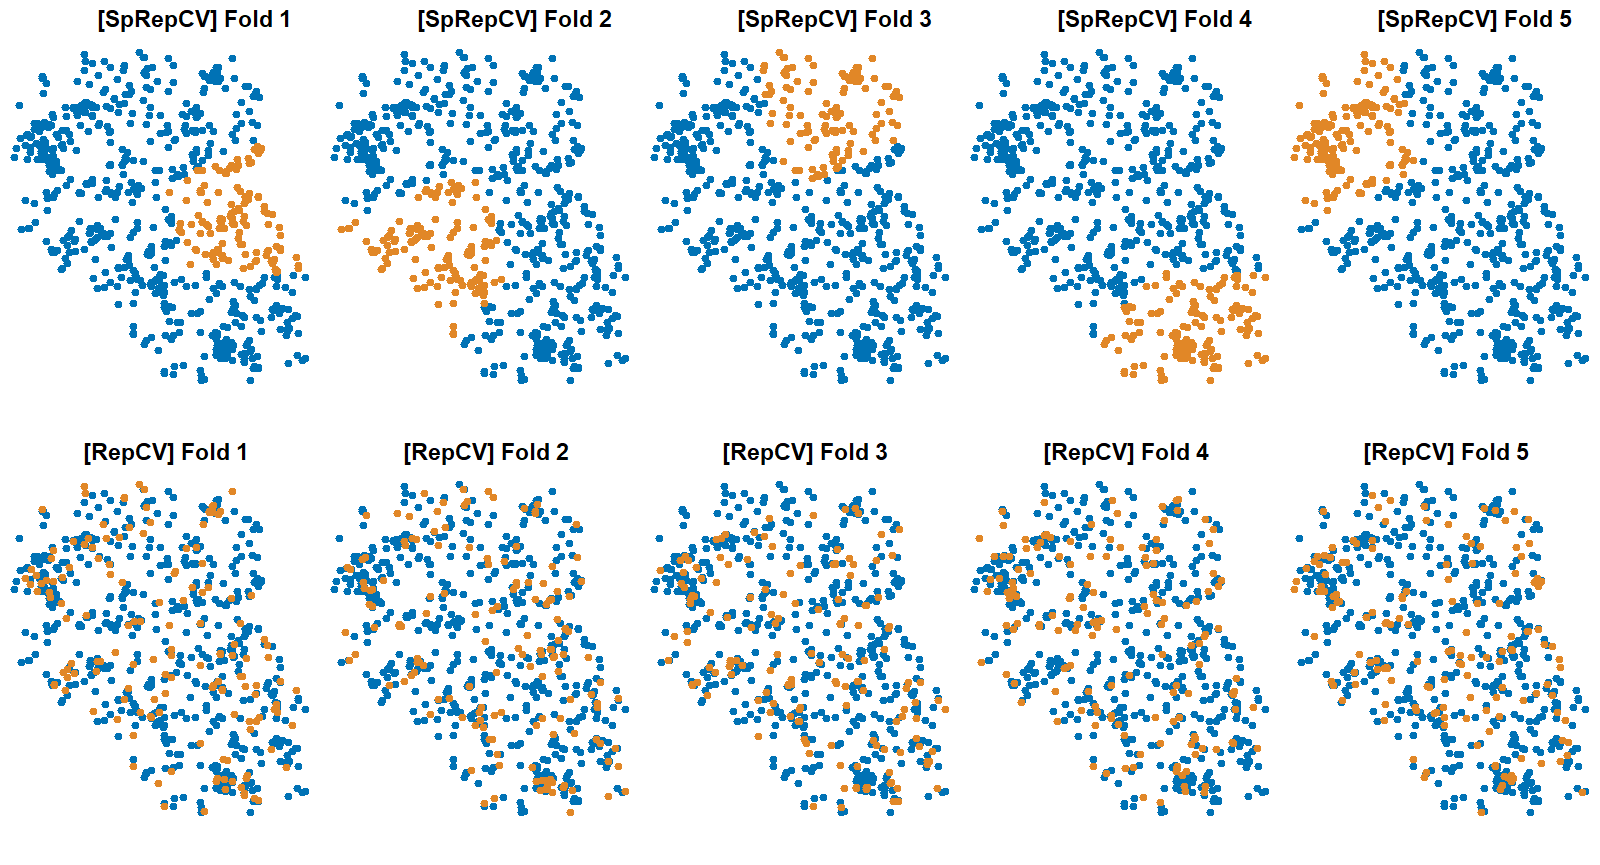
\includegraphics[width=1\textwidth,height=\textheight]{figures/spcv_plot.png}

}

\caption{\label{fig-rycina-spcv}Porównanie przestrzennego i losowego
podziału zbioru danych na potrzeby walidacji krzyżowej jednego
powtórzenia. Podział przestrzenny (górny rząd) i losowy (dolny rząd).
Opracowanie własne na podstawie
\href{https://mlr.mlr-org.com/articles/tutorial/handling_of_spatial_data.html}{kodu
Patricka Schratza}}

\end{figure}

Ocenę klasyfikatorów stworzonych dla każdego z wariantów (tabela
\ref{tbl-tabela-datasets}) przeprowadzono przy pomocy pięciu miar
jakości, przeznaczonych dla klasyfikatorów binarnych, wykorzystując
przestrzenną walidację krzyżową:

\begin{itemize}
\item
  precyzja (ang. \emph{precision}, inaczej \emph{positive predictive
  value}) - określa jaka część wyników wskazanych przez klasyfikator
  jako dodatnie jest faktycznie dodatnia
  \autocite{jaworski_2013_perfomance_measures}
\item
  czułość (ang. \emph{sensitivity}, inaczej \emph{recall} lub \emph{true
  positive rate}) - określa jaką część dodatnich wyników wykrył
  klasyfikator \autocite{jaworski_2013_perfomance_measures}
\item
  specyficzność (ang. \emph{specificity}, inaczej \emph{true negative
  rate}) - określa jaką część ujemnych wyników wykrył klasyfikator
  \autocite{jaworski_2013_perfomance_measures}
\item
  pole powierzchni pod krzywą (ang. \emph{Area Under Curve} lub
  \emph{Area Under the ROC Curve}, AUC lub AUROC) - oblicza obszar pod
  krzywą ROC, która graficznie przedstawia zależność pomiędzy czułością
  a specyficznością \autocite{jaworski_2013_perfomance_measures}. AUC
  ocenia prawdopodobieństwo, że losowo wybrana obserwacja pozytywna ma
  wyższe przewidywane prawdopodobieństwo niż losowo wybrana jednostka
  negatywna \autocite{R-mlr3measures}
\item
  \(F_{\beta}\) score (F-beta score) - ważona średnia harmoniczna
  pomiędzy precyzją i czułością, umożliwiająca ocenę balansu między
  czułością a precyzją, która w pewnym stopniu opisuje całościowo wynik.
  Miara ta nie uwzględnia wyników prawdziwie negatywnych
  \autocite{zygierewicz_2021_ml}
\end{itemize}

Wartości każdej z wymienionych miar jakości modelu zawierają się w
zakresie od 0 do 1, gdzie wartość 0 reprezentuje niską jakość modelu,
natomiast wartość 1 odzwierciedla wysoki poziom jakości. Wartości AUC
mieszczą się w zakresie od 0 do 1, gdzie wartość 0,5 lub niższa oznacza
oznacza model nie lepszy od losowego, a 1,0 -- doskonałe przewidywanie
obu klas. Wyższa wartość AUC wskazuje na lepszą moc predykcyjną modelu
\autocite{lovelace_2019_geocomputation}.

\hypertarget{waux17cnoux15bux107-zmiennych}{%
\section{Ważność zmiennych}\label{waux17cnoux15bux107-zmiennych}}

Ocena ważności zmiennych (ang. \emph{variable inportance}) może zostać
wykorzystana do poprawy i oceny jakości stworzonych modeli. Analizowanie
wpływu poszczególnych zmiennych na dokładność modelu umożliwia ocenę ich
istotności dla przewidywań. Stosowanie zmiennych o niskiej mocy
predykcyjnej może prowadzić do nadmiernego dopasowania (ang.
\emph{overfitting}) modelu lub obniżenia jego jakości. Dlatego ważny
jest wybór odpowiednich zmiennych do trenowania modelu, unikając na
przykład kolinearności predyktorów, czyli wysokiej korelacji między
zmiennymi. Celem określania ważności zmiennych i ich selekcji jest
zwiększenie mocy predykcyjnej modelu w kontekście analizowanego zjawiska
poprzez identyfikację silnie skorelowanych z nim zmiennych.

W lasach losowych ważność zmiennych można ocenić różnymi metodami, z
których dwie najpopularniejsze to miara zanieczyszczenia Giniego (ang.
\emph{Gini impurity}) oraz metoda oparta na permutacji
\autocite{R-Przewodnik}. W celu określenia wartości zmiennych
wykorzystywanych do identyfikacji farm fotowoltaicznych na podstawie
danych teledetekcyjnych, zastosowano metodę permutacji (ang.
\emph{permutation}), która może być również używana do upraszczania i
eksploracji modeli lub generowania wiedzy
\autocite{biecek_2021_model_analysis}.

Główną ideą metody opartej na permutacji jest pomiar tego, jak bardzo
zmieni się dopasowanie modelu, gdy usunięty zostanie wpływ wybranej
zmiennej lub grupy zmiennych. Jeśli zmienna jest istotna, permutacja jej
wartości skutkuje pogorszeniem jakości modelu. Im większa zmiana
dopasowania modelu, tym istotniejsza jest permutowana zmienna
\autocite{biecek_2021_model_analysis}.

Metoda oparta na permutacji została pierwotnie zaproponowana przez
\textcite{breiman_2001_rf} dla lasów losowych, jednak jej prostota
umożliwia zastosowanie permutacji do dowolnego modelu, a także
porównywanie ważności zmiennych pomiędzy modelami o różnych strukturach
\autocite{biecek_2021_model_analysis}.

\hypertarget{oprogramowanie}{%
\section{Oprogramowanie}\label{oprogramowanie}}

\hypertarget{qgis}{%
\subsection{QGIS}\label{qgis}}

QGIS \autocite{qgis}, to wieloplatformowe i wolne oprogramowanie o
otwartym kodzie źródłowym przeznaczone do przetwarzania danych
przestrzennych, rozwijane od 2002 roku
\autocite{hejmanowska_2020_dane,flenniken_2020_qgis}. Algorytmy
przetwarzania danych przestrzennych zebrane w oprogramowaniu QGIS
umożliwiają manipulację danymi rastrowymi oraz wektorowymi, a także
prowadzenie analiz i wizualizację wyników
\autocite{hejmanowska_2020_dane}. Oprogramowanie QGIS oferuje również
możliwość korzystania z wielu zewnętrznych programów, tzw. wtyczek (ang.
\emph{plug-in}) rozszerzających jego funkcjonalność
\autocite{hejmanowska_2020_dane}. W repozytorium wtyczek znaleźć można
narzędzia do zarządzania danymi, przetwarzania obrazów, wizualizacji,
czy wykonania dodatkowych zadań, takich jak np. nadawanie georeferencji
czy klasyfikacja zobrazowań satelitarnych
\autocite{hejmanowska_2020_dane}.

Oprogramowanie QGIS zostało wykorzystane w tej pracy do stworzenia
zestawu danych referencyjnych poprzez wizualną interpretację
ortofotomapy oraz mozaik satelitarnych. QGIS dostarcza zaawansowane
narzędzia do digitalizacji, umożliwiające rysowanie i edytowanie
obiektów wektorowych oraz pozwala na przeglądanie danych przestrzennych
dostępnych w Internecie za pomocą usług sieciowych, takich jak WMS, WMTS
czy XYZ Tiles.

\hypertarget{sentinel-1-toolbox-i-snap}{%
\subsection{Sentinel-1 Toolbox i SNAP}\label{sentinel-1-toolbox-i-snap}}

Przetwarzanie danych pochodzących z misji Sentinel-1 umożliwia zestaw
narzędzi S1TBX \autocite{s1tbx}, przeznaczony do przetwarzania danych
radarowych. Zestaw narzędzi Sentinel-1 Toolbox (S1TBX) zawiera narzędzia
do kalibracji, filtrowania plamek (tzw. efektu pieprzu i soli),
koregistracji, ortorektyfikacji, mozaikowania, konwersji danych,
polarymetrii czy interferometrii \autocite{sentinel-1-toolbox}.
Sentinel-1 Toolbox jest opracowywany dla ESA przez firmę Array we
współpracy z DLR, Brockmann Consult i OceanDataLab
\autocite{sentinel-1-toolbox}.

SNAP \autocite{snap}, czyli Sentinel Application Platform to platforma
oprogramowania rozwijana wspólnie przez firmy Brockmann Consult,
SkyWatch i C-S na zlecenie Europejskiej Agencji Kosmicznej (ESA),
przeznaczona do naukowego wykorzystania misji optycznych i mikrofalowych
Sentinel \autocite{snap-desktop,esa_snap}. Oprogramowanie SNAP zawiera
zestawy narzędzi do wizualizacji, przetwarzania oraz analizy danych
teledetekcyjnych, a także umożliwia tworzenie łańcuchów procesów
przetwarzania danych zdefiniowanych przez użytkownika
\autocite{hejmanowska_2020_dane,moskolai_2022_s1_workflow}.

\hypertarget{ux15brodowisko-jux119zyka-r}{%
\subsection{Środowisko języka R}\label{ux15brodowisko-jux119zyka-r}}

Czynności związane z końcowym przygotowaniem danych wejściowych oraz
bezpośrednio z uczeniem maszynowym zostały wykonane z wykorzystaniem
środowiska języka R \autocite{R-base}. R to wieloplatformowy język
programowania o otwartym kodzie źródłowym do obliczeń statystycznych i
wizualizacji danych. Dzięki dużej liczbie pakietów R obsługuje również
statystki geoprzestrzenne, modelowanie oraz wizualizację danych
przestrzennych \autocite{lovelace_2019_geocomputation}. W pracy
wykorzystane zostało zintegrowane środowisko programistyczne (ang.
\emph{Integrated Development Environment}, IDE) RStudio
\autocite{rstudio_team_2020_rstudio} przeznaczone dla języka R. Poza
standardowymi możliwościami środowiska R, w procesie pracy wykorzystane
zostały pakiety stworzone przez społeczność R w celu rozszerzenia
funkcjonalności tego języka. Do operacji na danych rastrowych
zastosowano pakiet \emph{terra} \autocite{R-terra}, natomiast do
przetwarzania danych wektorowych używany był pakiet \emph{sf}
\autocite{R-sf}. Obliczanie tekstury obrazu Sum Average wyprowadzonej z
macierzy współwystępowania poziomu szarości (ang. \emph{gray-level
co-occurrence matrix}, GLCM) zostało wykonane przy pomocy pakietu
\emph{GLCMTextures} \autocite{R-GLCMTextures}. Losowe generowanie danych
przestrzennych umożliwił pakiet \emph{spatstat.random}
\autocite{R-spatstat.random} z rodziny pakietów \emph{spatstat}
\autocite{R-spatstat}. Do przeprowadzenia analizy oraz predykcji opartej
o elementy uczenia maszynowego wykorzystano pakiet \emph{mlr3}
\autocite{R-mlr3}, w ramach którego użyty został algorytm lasów losowych
zaimplementowany w pakiecie \emph{ranger} \autocite{R-ranger}. Do
obliczeń związanych z teksturami obrazu oraz uczeniem maszynowym
wykorzystano pakiet \emph{future} \autocite{R-future}, umożliwiający
równoległe (wielowątkowe) przetwarzanie wyrażeń R, skracające czas
realizacji zadań w stosunku do przetwarzania sekwencyjnego.

\bookmarksetup{startatroot}

\hypertarget{sec-wyniki}{%
\chapter{Wyniki}\label{sec-wyniki}}

\hypertarget{ocena-jakoux15bci-modeli-1}{%
\section{Ocena jakości modeli}\label{ocena-jakoux15bci-modeli-1}}

\hypertarget{waux17cnoux15bux107-zmiennych-1}{%
\section{Ważność zmiennych}\label{waux17cnoux15bux107-zmiennych-1}}

\hypertarget{wizualna-kontrola-wynikuxf3w-klasyfikacji}{%
\section{Wizualna kontrola wyników
klasyfikacji}\label{wizualna-kontrola-wynikuxf3w-klasyfikacji}}

\bookmarksetup{startatroot}

\hypertarget{podsumowanie}{%
\chapter{Podsumowanie}\label{podsumowanie}}

Podsumowanie pracy jest w pewnym sensie znacznie rozbudowanym
abstraktem. Należy wyliczyć i opisać osiągnięcia uzyskane w pracy
dyplomowej. Tutaj jednak (w przeciwieństwie do np. rozdziału
\ref{sec-wprowadzenie}) należy przechodzić od szczegółu do ogółu - co
zostało stworzone/określone, jak zostało to zrobione, jakie ma to
konsekwencje, itd.

Ten rozdział powinien też zawierać opis kwestii, których nie udało się
rozwiązać w pracy dyplomowej (i dlaczego się nie udało) oraz pomysły na
przyszłe ulepszenie uzyskanych wyników lub dalsze badania.

\printbibliography[heading=bibintoc, title=Bibliografia]

\end{document}
